\documentclass[a4paper,oneside,article,table]{article}

%encoding
%--------------------------------------
\usepackage[T1]{fontenc}
\usepackage[utf8]{inputenc}
%--------------------------------------

%Portuguese-specific commands
%--------------------------------------
\usepackage[brazil]{babel}
%--------------------------------------

%Hyphenation rules
%--------------------------------------
\usepackage{hyphenat}
\hyphenation{mate-mática recu-perar}
%--------------------------------------

%Page formatting
%--------------------------------------
\usepackage[a4paper, total={6in, 8in}]{geometry}
\usepackage{multicol}
\usepackage{indentfirst}
\usepackage{enumitem}
%--------------------------------------

%Plotting Graphs
%--------------------------------------
\usepackage{tikz}
\usetikzlibrary{positioning}
\usetikzlibrary{graphs}
%--------------------------------------

%Misc
%--------------------------------------
\usepackage[bottom]{footmisc}
\usepackage{amsmath}
\usepackage{mathtools}
\usepackage{graphicx}
\usepackage{array}
\usepackage{microtype}
\usepackage{xparse}
\usepackage{booktabs}
\usepackage{float}
\usepackage{caption}
\usepackage{textcomp}
\usepackage{mdwlist}
\usepackage{subcaption}
%--------------------------------------


\title{Anotações MC658}
\author{Eduardo M. F. de Souza}
\date{\today}

\definecolor{light gray}{gray}{0.8}
\renewcommand{\arraystretch}{1.3}

\renewcommand{\P}{\mathcal{P}}
\newcommand{\NP}{\mathcal{NP}}
\newcommand{\NPC}{\mathcal{NP}\textit{-Completo}}
\frenchspacing
\raggedbottom{}
%\raggedright{}


\begin{document}

\pagenumbering{gobble}
\maketitle

\pagenumbering{arabic}

\tableofcontents
\newpage

\section{Classes de Complexidade}

\subsection{Características}

\begin{itemize}

    \item São classes que contém problemas, e, problemas que contém determinadas características em comum;
    \item A maior parte dos algoritmos vistos até então têm tempo polinomial --- $O(n^k)$ onde $k$ é constante e $n$ é o tamanho da entrada;
    \item Nem todo problema admite um algoritmo polinomial para resolvê-lo. \par
        Exemplo: problema da parada, no qual sequer admite um algoritmo, independente do tempo; programa para predizer se um algoritmo pode entrar em \textit{deadlock} ou não em uma máquina genérica;
        \begin{itemize}
        \item É \textbf{tratável} se admite um algoritmo polinomial;
        \item E \textbf{intratável} se não admitir um algoritmo polinomial (pode admitir um algoritmo exponencial);
    \end{itemize}

\end{itemize}

\subsection{$\P$, $\NP$ e $\NPC$}

\begin{itemize}
    \item \textbf{$\P$:} Classe em que os problemas que possuem algoritmos que os resolvem em tempo polinomial;
    \item \begin{multicols}{2}
            \textbf{$\NP$:} Classe em que os problemas admitem um algoritmo polinomial que verifiquem instâncias do problema. \par
            Um exemplo é o Ciclo Hamiltoniano:
            \begin{description}
                \item\textit{Entrada:} Grafo simples $G=(V,E)$.
                \item\textit{Saída:} Existe ou não um ciclo que passa por cada vértice exatamente uma vez.
                \item\textit{Verificação:}
                    \par (1,2,3,6,4,5) \textrightarrow{} não é uma solução válida;
                    \par (1,2,3,4,5,6) \textrightarrow{} é uma solução válida;
            \end{description}
            \vfill

        \begin{center}
            \begin{tikzpicture}
                \graph[nodes={circle, draw}, branch down = 1.5cm, grow right = 1.5cm]{
                    2 -- 1 ,
                    2 -- 3 -- 1,
                    3 -- {4 -- 6 -- 1},
                    4 -- 5 -- 6 -- 3;
                };
            \end{tikzpicture}
        \end{center}

    \end{multicols}

    \item \textbf{$\NPC$:} Todo problema desta classe está em NP.\@Problemas NPC têm a característica de, se algum deles admitir um algoritmo polinomial, então automaticamente todos os problemas de NP possuem um algoritmo polinomial;
    
\end{itemize}

\begin{figure}
    \centering
    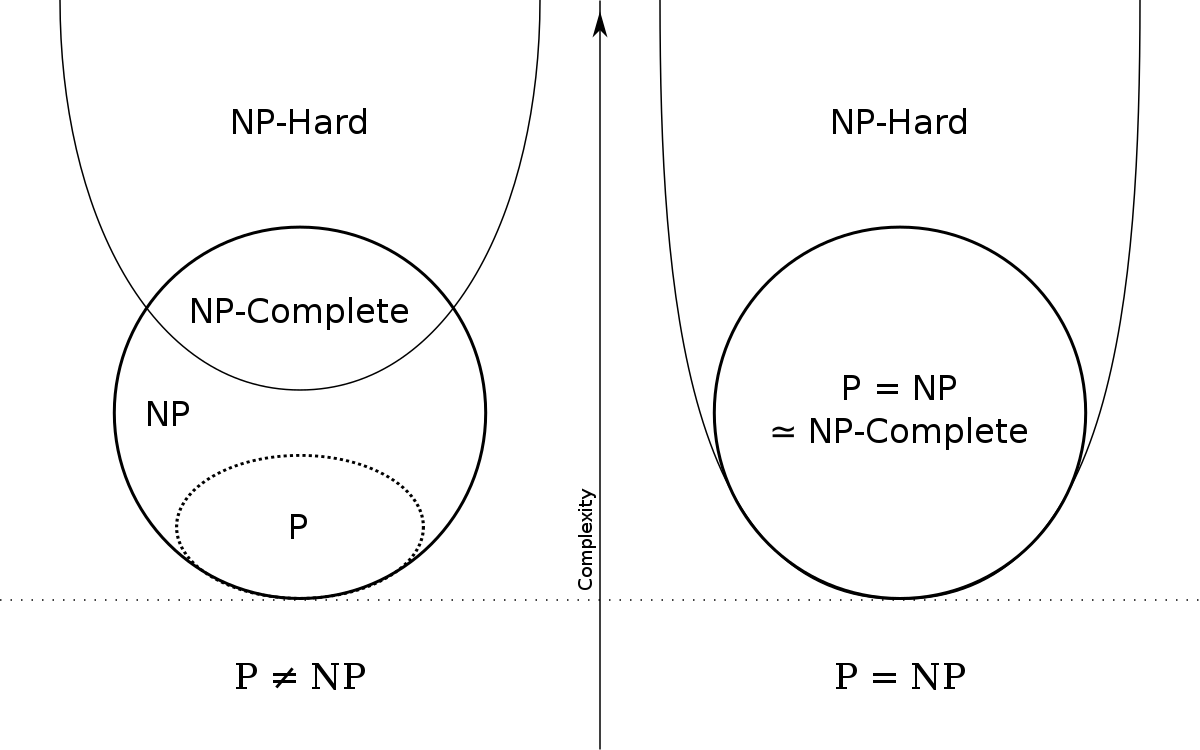
\includegraphics[width=0.7\textwidth]{imgs/P_np_np-complete_np-hard.png}
    \caption*{\centering{$\P \leq \NP~|~\NP \in \P$ é uma questão em aberto. Desde 1970 até hoje um importante problema aberto é se $\P = \NP$.}}
    
\end{figure}
\subsection{Problemas de Decisão}
Resposta deve ser de \textbf{Sim (1)} ou \textbf{Não (0)}.

\paragraph{Exemplo:} Da versão de decisão do problema do menor caminho em um grafo:
\begin{description}
    \item \textit{Entrada:} $G= (V,E)$ com pesos nas arestas, valor $k$, e $u,v \in V$
    \item \textit{Pergunta:} Existe caminho $u \to v$ com custo $\leq k$?
\end{description}


\subsubsection{Formalização matemática de um problema}
\begin{itemize}
    \item Um problema será definido como um lingagem sobre um alfabeto $\Sigma$;
    \item Usaremos $\Sigma = {0,1}$ (binário);
    \item Dado um problema $Q$, qualquer instância desse problema será codificada como uma string de $0$s e $1$s;
    \item Uma linguagem \underline{$L$} de $\Sigma$ é um \underline{conjunto de strings} formadas com os símbolos de $\Sigma$.\\
        Notação:
        \begin{itemize}
            \item $E$: string vazia
            \item $\emptyset$: Uma linguagem vazia
            \item $\Sigma^*$: Todas as possíveis strings que podem ser escritas com os símbolos de $\Sigma$.\\
                Exemplo: $\Sigma^* = \{E, 0, 1, 00, 01,~\ldots\}$
        \end{itemize}
    \paragraph{Observação:} Qualquer lingaguem $L$ é tal que $L$ contem em $\Sigma^*$.
\end{itemize}

Um problema de decisão $Q$ será visto como uma linguagem que contém todas as strings de $\Sigma^*$ que corresponde às instâncias de $Q$ cuja resposta é sim.

Exemplo:
\begin{description}
    \item Ciclo-Hamiltoniano = \{ $\langle G = (V, E)\rangle$ tal que $G$ possui um Ciclo Hamiltoniano\}
    \item $\langle~\rangle$: Notação que corresponde à codificação da instância como uma string.
\end{description}

\subsubsection{Operações sobre Linguagens}
\begin{itemize}
    \item \textbf{União:} $L_1\cup L_2 = \{ s : s \in L_1 \textrm{ ou } s \in L_2\}$
    \item \textbf{Concatenação:} $L_1L_2 = \{ x, y : x \in L_1 \textrm{ ou } y \in L_2\}$
    \item \textbf{União:} $L_1 \cap L_2 = \{ s : s \in L_1 \textrm{ ou } s \in L_2\}$
\end{itemize}

\subsection{Algoritmos}
\begin{itemize}
    \item Uma entrada para um algoritmo $A$ é qualquer string de $\Sigma^*$;
    \item Um algoritmo aceita $s\in\Sigma^*$ se $A(s)=1$;
    \item Um algoritmo rejeita $s\in\Sigma^*$ se $A(s)=0$;
    \item Um algoritmo aceita uma linguagem $L$ se $\forall s \in L \Rightarrow A(s)=1$.
        Para strings $s \notin L \Rightarrow A(s) \neq 1$ o algoritmo pode não parar --- entra em loop infinito;
    \item $A$ é um algoritmo que decide uma linguagem $L$ se 
        $\begin{cases}
            \forall s \in L \Rightarrow A(s) = 1\\
            \forall s \notin L \Rightarrow A(s) = 0
        \end{cases}$
    \item Uma linguagem é \textbf{aceita} em tempo polinomial se existe um algoritmo polinomial $A$ que \textbf{aceita} $L$;
    \item Uma linguagem é \textbf{decidida} em tempo polinomial se existe um algoritmo polinomial que \textbf{decide} $L$;

\end{itemize}

    \subsection{Definição da classe $\P$}

        \[\P = \{ L \in \Sigma^*~|~L \textrm{ é decidido em tempo polinomial} \}\]

        \paragraph{Teorema:} $\P$ é o conjunto de todas as linguagens decididas em tempo polinomial.
        \[\P = L \in \Sigma^*~|~L \textrm{ é aceita em tempo polinomial} = \P'\]

        \paragraph{Prova:}
        \begin{description}
            \item \textbf{Contido:}
                \begin{description}
                    \centering{
                    \item Seja $L$ decidida em tempo polinomial $\Rightarrow$
                    \item $\Rightarrow$ $\exists$ um algoritmo $A$ polinomial que decide $L$ $\Rightarrow$
                    \item $\Rightarrow$ $A$ aceita $L$ em tempo polinomial;
                    }
 
                \end{description}
            \item\textbf{Contrário de contido:}
                \begin{description}
                    \centering{
                    \item Seja $L$ aceita em tempo polinomial $\Rightarrow$
                    \item $\Rightarrow$ $\exists$ um algoritmo $A : s \in L~|~A(s) = 1$ em tempo $c\times|s|^k$ (polinomial) onde $c$ e $k$ são constantes;
                    }

            \end{description}
    \end{description}

        Existe um algoritmo $A'$ que simula $A$ por $c\times|s|^k$ passos. Se $A(s)=1$, então $A'(s) = 1$ e caso $A(s)$ não responda nada (ou zero) então $A'(s) = 0$ $\Rightarrow$  $L$ é decidida em tempo polinomial.

        %==============================================================================

        \paragraph{Problema de Decisão:}
        \begin{align*}
            \Sigma &= \{0,1\}\\
            \Sigma^*&=\{E, 0, 1, 00, 01, \ldots\}
        \end{align*}

        Problema $Q \subseteq \Sigma^*~|~x \in Q \iff$ a resposta para instância $x$ é sim.

        Algoritmo $A$ que decide uma linguagem $L \subseteq \Sigma^*$:
        
        \[A(x) = \begin{cases}
            1,~\forall x \in L\\
            0,~\forall x \notin L
        \end{cases}\]
        \[P = \{L \subseteq \Sigma^*~|~\exists \textrm{ um algoritmo } A \textrm{ que decide } L \textrm{ em tempo polinomial}\}\]


        \subsection{Verificação}

        Ciclo Hamiltoniano = \{<$G=(V,E)>$ onde G é um grafo simples e G possu um ciclo que passa por cada vértice exatamente uma vez}

        Algoritmo Verificador para uma linguagem $L \subseteq \Sigma^*$.
        $A(x, y)$ onde x é uma instância de L e y é outra string que chamamos de certificado.

        \begin{enumerate}
            \item Se $x \in L$ então $\exists y \in \Sigma^* / A(x,y) = 1$
            \item Se $x \notin L$ então $\forall y \in \Sigma^*  / A(x,y) \neq 1$
        \end{enumerate}

        \subsection{Algoritmo Verificador para Ciclo Hamiltoniano}
        A(G, sequência vertical ($v_1, v_2, \ldots, v_n$)) -> Verificar que correspondem a todos os vértices do grafo exatamente uma vez.
            For v \in (v_1, v_2, \ldots, v_n)
            If v \notin G return 0
            For i = 1 to n-1
            if(v_i,v_{i+1}) \notin G return 0
            if(v_1, v_n) \not in G return 0
            return 1

            Se G \in Ciclo-Hamiltoniano, então existe uma sequência de vérticas que corresponde ao ciclo e usamos isto como certificado.

            Se G \not in Ciclo-Hamiltoniano então na checagem das arestas, para qualquer sequência de vértices, uma aresta estará faltando.

            Um algoritmo A(x,y) verifica L \subseteq \Sigma^* em tempo polinomial se A executa em tempo polinomial em |x| e |y| e:
            \begin{enumerate}
                \item Se x \in L, então \exists y \in \Sigma^* / |y| = O(|x|^k) para k constante. A(x,y)=1
                \item Se x \notin L então \forall y \in \Sigma^* / |y| \ in O(|x|^k) temos que A(x,y) \neq 1

            \end{enumerate}

    \subsection{Classe NP}

        NP = \{L \subseteq \Sigma^* / \exists A(x,y) polinomial que verifica L\}

        Questão em aberto: P = NP?

        Exercício> P \subseteq NP

        Seja L \in P (mostrar que L \in NP) \arrowright Existe algoritmo A(x) que decide L em tempo polinomial.

        A1(x,y)
            return A(x)

        \begin{enumerate}
            \item $x \in L$, então usando $y = E$ temos que $A'(x,y) = 1$ e $|y| \in O(|x|^k)$
            \item $x \notin L$, então $A(x) = 0 \rightarrow A1(x,y) = 0$ independente do $y$.
        \end{enumerate}

    \subsection{Classe co-NP}

        Dado $L \subseteq \Sigma^*$ definimos o complemento de $l$ como
        \[\overline{L} = \Sigma^* \backslash L\]
        co-NP $= \{L \subset \Sigma^* / \overline{L} \in$ NP\}

        Instintivamente, co-NP contém as lingaguens para as quais existe algoritmo verificador polinomial para instâncias "não" do problema.
        $L \in $ co-NP se existe um algoritmo polinomial $A(x,y)$, dois quais $x$ é instância e $y$ é um certificado, onde:
        \begin{enumerate}
                \item $x \not in L, \exists y \in \Sigma^* / |y| = O(|x|^k)$ e $A(x,y) = 1$
                \item $x \in L, \forall y \in \Sigma^* / |y| = O(|x|^k)$ e $A(x,y) \neq 1$
        \end{enumerate}

        Primos \{ <n> N é um inteiro positivo e é primo\}

        Primos \in co-NP pois podemos criar um algoritmo que para cada n \neq Primos \rightarrow \exists um divisor d de n que serve como certificado polinomial que n não é primo.

        Questão em aberto> NP = co-NP ?

        Exercício: p \subseteq NP \cap co-NP (Acabamos de ver qie P \subseteq NP)
        Mostrar P \subseteq co-NP! Seja L \in P \rightarrow existe um algoritmo polinomial A(x) que decide L.

        A'(x,y)
            if A(x) == 1 return 0
            if A(x) == 0 return 1

        \begin{enumerate}
            \item $x \notin L$ então A(x,E) = 1 em tempo polinomial
            \item $x \in L$ então A(x,y)=0 independe do y.
        \end{enumerate}

        \subsection{Possíveis Relações entre estas Classes}

        P = NP \rightarrow P = NP = co-NP
        P \neq NP \rightarrow P \in NP = co-NP
        P \neq NP \rightarrow P = NP \bigcap co-NP, NP \neq co-NP
        p \neq NP \rightarrow P \subset NP \bigcap co-NP, NP \neq co-NP

        % ============= Curiosidade
        $n = p_{1}^{j_1} \times p_{2}^{j_2} \times \ldots \times p_{q}^{j_q}$
        Qualquer $n \in \Z^+$ possui uma fatoração única em primos distintos.

        RSA (ninguém consegue achar um fator de n em tempo polinomial)

        Fatoração: Dado n e m \leq n existe um fator p de n tal que $p \leq m$

        Fatoração \in P? Ninguém sabe.

        Fatoração \in co-NP e Fatoração \in NP.

        Fatoração \in NP: Dado (n,m) \in Fatoração, basta usar como certificado um fato p \leq m!
        Fatoração \in co-NP: (n,m) \notin Fatoração \rightarrow $\nexists$ fator primo p\leq m tal que p divida n. Meu certificado é uma fatoração de n em primos $p_{1}^{j_1}, p_{2}^{j_2}, \ldots, p_{q}^{j_q}$

        \begin{enumerate}
            \item Verificar que a multiplicação do valor n
                n = p_{}^{}p_{}^{}p_{}^{}

            \item Verificar que cada p_j é um número primo (feito em tempo polinomial com AKS de 2006)
            \item Verificar que cada p_j \ge m
        \end{enumerate}

        \subsection{Reduções Polinomiais}
        \textbf{Definição:} sejam $L_1, L_2 \subseteq \Sigma^*$ duas linguagens. Dizemos qye $L_1$ se reduz para $L_2$ em tempo polinomial se:
        \begin{enumerate}
            \item Existe um algoritmo $F$ que tranforma a instância $x_1$ de $L_1$ em instâncias $x_2 = F(x_1)$ de $L_2$ em tempo $O(|x_1|^k)$, $k$ constante;
            \item $x_1 \in L_1 \iff F(x_1) = x_2 \in L_2$;
        \end{enumerate}

        \textbf{Pergunta:} Dado $x_1 \notin L_1$, é possível $F(x_1) = x_2 \in L_2$?
        \textbf{R:} Não é possível!

        \subsubsection{Lema 34.3}
        Sejam $L_1, L_2 \subseteq \Simga^*$ tal que $L_1 {\leq}_p L_2$. Se $L_2 \in P$, então $L_1 \in P$

        Como $L_2 \in P \rightarrow \exists$ algoritmo polinomial $A_2$ que decide $L_2$. Podemos construir:
        A_1(x_1):
        x_2 = F(x_1)
        return A_2(x+2)

        Como $L_1 {\leq}_p L_2$ existe o algoritmo de redução $F$ de $L_1$ pra $L_2$.

        \begin{itemize}
            \item $A_1$ executa em tempo polinomial (tanto $A_2$ quanto $F$ têm tempo polinomial)
            \item 
                \begin{enumerate}
                    \item Dado $x_1 \in L_1 \rightarrow F(X_1) = x_2 \in L_2$ e $A_2(x_2) = 1 \rightarrow A_1(x_1) = 1$
                    \item Dado $x_1 \notin L_1 \rightarrow F(x_1) = x_2 \notin L_2$ e $A_2(x_2) = 0 \rightarrow A_1(x_1) = 0$
                \end{enumerate}
        \end{itemize}

        \subsection{NP-Completo (NPC)}
        Uma linguagem $L \in \textrm{NPC}$ se ela satisfizer:
        \begin{enumerate}
            \item $L \in \textrm{NP}$
            \item $\forall L' \in \textrm{NP}$ então existe redução polinomial de $L'$ para $L$, $L1 {\leq}_p L$
        \end{enumerate}

        \textbf{Obs:} As linguagens (problemas) que só satisfazem a condição (2) pertencem à classe NP_Difícil.

        \subsection{Teorema 34.4} Seja $L \in \textrm{NPC}$. Se $L \in \textrm{P}$, então $\forall L' \in \textrm{NPC}$. Temos que $L' \in \textrm{P}$

        \textbf{Prova:} Seja $L' \in \textrm{NP}$ um problema qualquer. Sabemos que $L \in \textrm{NPC} \rightarrow L' {\leq}_p L$.\\
        Sabemos que $L \in \textrm{P}$, então, pelo lema anterior, $L' \in \textrm{P}$! 

        % Wtf ==============================
        \[P_1 \in \textrm{NPC}\]
        \[\forall L \in \textrm{NP},~L {\leq}_p P_1\]
        \[P_2,~P_1 {\leq}_p P_2\]

        Ao mostrarmos que um problema $L_1 \in NPC$, estamos dando fortes indícios que $L_1$ não admite um algoritmo polinomial.
        Melhor resolver $L_1$ com técnicas para lidar com problemas NP-Difíceis.

        \subsection{Teorema de Cook (1971)}
            \subsubsection{Problema SAT}
                Dadas variáveis booleanas $x_1,~\ldots,~x_n$ e uma fórmula sobre elas com operadores $\lor,~\land,~\ne,~\rightarrow,~\iff$, existe uma atribuição para $x_1,~\ldots, x_n$ tal que $f$ fica verdadeira?

            \subsubsection{Circuit-SAT}
            Portas lógicas: not, or, and (podem ter mais entradas).

            Dado um circuito lógico com entradas $x_1,~\ldots,~x_n$ e uma única saída, existe uma atribuição para $x_1,~\ldots,~x_n$ tal que a saída do circuito é verdadeira?

            Os circuitos considerados não possuem \textit{loop}?

            %{X1, X2} -> Or -> X4
            %(X1, X2, not X3} -> And -> X5
            %{X4, not not X3} -> Or -> X6
            %{not not X3, X5} -> And -> X7
            %{X6, X7, X5} -> And -> Final

            \subsubsection{Circuit-SAT $\in$ NP}
            Vamos mostrar que Circuit-SAT é NP-Difícil.

            %Alg/Prog <-> CPU
            %Entrada <-> CPU
            %PC <-> CPU
            %Mem <-> CPU
            %Controle <-> CPU
            
            Uma máquina é construída com vários circuitos lógicos.

            Seja $L \in \textrm{NP}$, queremos mostrar que existe $L~{\leq}_p$ Circuit-SAT.
            Sabemos que existe um algoritmo $A(x,y)$ verificador polinomial para $L$.
            \begin{enumerate}
                \item Se $x \in L,~\exists y$ tamanho polinomial tal que $A(x,y) = 1$;
                \item Se $s \notin L,~\forall y$ tamanho polinomial tal que $A(x,y) \neq 1$;
            \end{enumerate}
            Dado $x$, assumimo que $A$ executa no máximo $c_1|x|^{k_1}$ passos ($c_1,~k_1$ são constantes) e $|y| \leq c_2|x|^{k_2}$, onde $c_2$ e $k_2$ são constantes.

            Podemos \"usar\" o computador para executar o algoritmo A
        
            %A <-> CPU
            %Alg/Prog <-> CPU
            %Entrada <-> CPU
            %PC <-> CPU
            %Mem <-> CPU
            %Controle <-> CPU

            %A -> CPU
            %Alg/Prog -> CPU
            %Entrada -> CPU
            %PC -> CPU
            %Mem -> CPU
            %Controle -> CPU
            %CPU -> {PC_2, Mem_2, Controle_2}

            Dado $x$ uma instância de $L$. Montamos um circuito l[ogico com $c_1|x|^{k_1}A$ cópias do \"computador\" que faz a simulação do algoritmo verificador $A$;
            Tamanho dos circuitos representando, $A$, PC, Mem e Controle são constantes.
            Assumimos que $x$ é setado fixo com seu próprio valor.
            A única entrada deste circuito é o $y$;
            Dado $x \in \Sigma^*$ instância de $L$, construímos um circuito C \underline{em tempo polinomial}!
            \begin{enumerate}
                \item Se $x \in L$ então $\exists y$ polinomial tal que $A(x,y) = 1$. Este mesmo $y$ serve como entrada para o circuito C, deixando ele satisfazível \rightarrow C $\in$ Circuit-SAT
                \item Se $x \not in L$ então $\forall y$ de tamanho polinomial, $A(x,y) \neq 1 \forall$ entrada $y$ de C \rightarrow C nunca será satisfazível \rightarrow C $\notin$ Circuit-SAT.
            \end{enumerate}

            \subsection{Provas de NP-Completude}
            Mostramos que o Circuit-SAT é  NP-Completo:
            \begin{enumerate}
                \item Circuit-SAT $\in$ NP;
                \item $\forall L \in$ NP existe redução em tempo polinomail de $L /{leq}_{pol}$ Circuit-SAT.\\
                    % L         F(x)        Circuit-SAT
                    % x --------------------------> C
                    $x \in L \iff C \in$ Circuit-SAT
            \end{enumerate}

            Vale a transitividade para {\leq}_{pol}:
            \begin{equation*}
                P_1 {\leq}{_pol} P_2~\mathrm{e}~P_2 {\leq}{_pol} P_3 \rightarrow P_1 {\leq}{_pol} P_3
            \end{equation*}

            \subsubsection{SAT}
            Fórmula booleana $f$ com variáveis $x_1,~\ldots,~x_n$ e operadores $\lnot$, $\lor$, $\land$, $\rightarrow$, $\iff$. 
            Existe atribuição para $x_1,~\ldots,~x_n$ tal que $f$ fica verdadeiro.
            \[f = (x_1 \rightarrow x_2) \lor \lnot ( (\lnot x_1 \iff x_3) \lor x_4) \land  \lnot x-2\]

            SAT = \{ $<f>$ onde $f$ é uma fórmula lógica que possui atribuição verdadeira\}

            Para mostrar que SAT é NP-Difícil (condição 2 de NPc) faremos Circuit-SAT ${\leq}_{pol}$ SAT
            $\forall L \in$ NP, sabemos que $L {\leq}_{pol}$ Circuit-SAT e, por transitividade, teremos $L {\leq}_{pol}$ SAT.

            \begin{table}
                \begin{tabular}{c c c c}
                        $x_1$ & $x_2$ & $x_1 \rightarrow x-2$ & $x_1 \iff x_2$\\
                        0 & 0 & 1 & 1\\
                        0 & 1 & 1 & 0\\
                        1 & 0 & 0 & 0\\
                        1 & 1 & 1 & 1\\
                \end{tabular}
            \end{table}

            \paragraph{Teorema 34.9:} SAT $\in$ NP-Completo.
            Prova:
            \begin{enumerate}
                \item SAT $\in$ NP (fica como exercício);
                \item Mostrar que Circuit-SAT ${\leq}_{pol}$ SAT:
                    \begin{description}
                        \item $C \in$ Circuit-SAT $\iff f \in$ SAT.
                        \item Dado um circuito $C$ qualquer, vamos construir a fórmula $f$ em tempo polinomial onde vale o item anterior.

                            % circuito lógico do qual tirei foto

                        \item Dado $c$ além das variáveis de entrada, criamos uma nova variável para saíde de uma porta lógica do circuito.
                        \item Escreveremos uma cláusula para cada porta lógica.\\
                            Exemplo: $(x_5 \iff (x_1 \lor x_2))$

                        \item Cada cláusula só pode ser verdadeira quando o valor de variável de saída da porta lógica correspondem ao que é computado pela porta lógica.
                        \item A formula $f$ será um \textit{and} de todas as cláusulas correspondentes a cada uma das portas lógicas mais a última variável de saída do circuito.
                            \begin{align*}
                                f = x_{10} &\land (x_4 \iff (\lnot x_3))\\
                                &\land (x_5 \iff (x_1 \lor x_2))\\
                                &\land (x_6 \iff \lnot x_4)\\
                                &\land (x_7 \iff (x_1 \land x_2 \land x_4))\\
                                &\land (x_8 \iff (x_5 \lor x_6))\\
                                &\land (x_9 \iff (x_6 \lor x_7))\\
                                &\land (x_{10} \iff (x_7 \land x_8 \land x_9))
                            \end{align*}
                    \end{description}
            \end{enumerate}
            
            Dado $C$ qualquer podemos construir $f$ em tempo proporcional ao número de portas lógicas em C e, portanto, em tempo polinomial.
            \begin{enumerate}
                \item Suponha que $C \in$ Circuit-SAT:
                    \begin{description}
                        \item \rightarrow Existe uma atribuição para as variáveis de entrada que deixa $C$ verdadeiro.
                        \item Simulando essa entrada no circuito, computamos o valor de saída para cada porta lógica e atribuímos esse valor para a variável de saída correspondente da porta lógica \rightarrow cada cláusula corresponde a uma porta lógica fica verdadeira.
                        \item Além disso, a saída de $C$ é verdadeira \rightarrow a variável de saída final é verdadeira \rightarrow $f$ fica verdadeiro.
                            \[f \in \text{SAT}\]
                    \end{description}

                \item $f \in$ SAT (temos que mostrar que $C$ que deu origem a $f$ é tal que $C \in$ Circuit-SAT)\\
                    $f \in$ SAT \rightarrow existe atribuição para variávekd e $f$ que deixa $f$ verdadeiro. Usamos os valores das variáveis de entrada em $f$ como a entrada correspondente em $C$.\\
                    Para cada porta porta lógica de C, o seu valor de saída é igual ao valor da variável de saída da cláusula correspondente a essa porta lógica.\\
                    O valor de saída de cada clausula é igual a porta lógica correspondente quando damos essa entrada.\\
                    Como em $f$ a saída final é verdadeira e ela de deve ser igual a saída da última porta lógica \rightarrow A saída do circuito é 1 \rightarrow $C \in$ Circuit-SAT.
            \end{enumerate}

            \subsection{3 CNF-SAT}
            Uma fórmula que é uma conjunção (and) de cláusulas e cada cláusula é uma disjunção (or) de exatamente três literais ($x_i$ ou $\overline{x_i}$).\\
            Existe atribuição verdadeira?A\\
            Exemplo: $f = (x_1 \lor \overline{x_2} \lorr x_3)\land(x_4 \lor \overline{x_5} \lor x_1)\land(x_2 \lor \overline{x_3} \lor \overline{x_4})$

            \boxed{Teorema: 3CNF-SAT é NP-Completo}
            Prova:
            \begin{enumerate}
                \item 3CNF-SAT $\in$ NP (exercício)
                \item 3CNF-SAT $\in$ NP-Difícil.\\
                    Faremos SAT ${\leq}_{pol}$ 3CNF-SAT.
                    A partir de $f_1$ de SAT, construiremos um $f_2$ do 3CNF-SAT.
                    \[f_1 - ((x_1 \rightarrow) \land \lnot ((\lnot x_1 \iff x_3) \land \lnot x_2\]
                    \begin{description}
                        \item Construímos uma árvore de avaliação da fórmula onde as folhas são os literais da fórmula, nós são os operadores lógicos da fórmula.
                    
                            %Grafo que eu tirei foto
                        \item Criamos $f_1'$ equivalente a $f_1$ que corresponde à avaliação da árvore construída.
                            \begin{align*}
                                f_1' = y_1 &\land (y_1 \iff (y_2 \land \lnot x_2))\\
                                &\land (y_2 \iff (y_3 \or y_4))\\
                                &\land (y_3 \iff (x_1 \rightarrow x_2))\\
                                &\vdots\\
                                & \land (y_5 \iff \lnot x_6)
                            \end{align*}

                        \item Cada cláusula em $f_1$ tem no máximo 3 literais (cada operador lógico tem no máximo 2 entradas e tem uma saída);
                        \item $f_1'$ pode ser computado em tempo polinomial.
                    \end{description}

                    \textbf{Deixar cada cláusula na CNF}

                    \begin{description}
                        \item Para cad cláusula $f_i'$ de $f_1$, construímos uma tabela verdade.\\
                            Exemplo: $(y_1 \iff (y_2 \land \overline{x_2})) = f_i'$
                            % tabela y_1 y_2 x_2 f_i'
                        \item POdemos escrever fórmulas na DNF (forma normal disjuntiva equivalente à $f_1'$
                            \[f_i'' = (\overline{y_1} \land \overline{y_2} \land \overline{x_2}) 
                                \lor (\overline{y_1} \land \overline{y_2} \land x_2) 
                                \lor \ldots\]

                        \item \boxed{Criar $\overline{f_i''}$ na DNF que corresponde a $f_i$}
                            \[\overline{f_i'} \approx \overline{f_i''} = 
                                (\overline{y_1} \land y_2 \land \overline{x_2})
                                \lor (y_1 \land \overline{y_2} \land \overline{x_2})
                                \lor (y_1 \land \overline{y_2} \land x_2)
                                \lor (y_1 \land y_2 \land x_2))
                            \]

                            % Negar a expressão de cima e inverter tudo
                            Aplicando De'Morgen, obtemos:

                        \item A partir de $f_1'$, construímos $f_1''$ equivalente e que está na CNF e isso em tempo polinomial. Cada cláusula de $f_1'$  temos no máximo 3 variáveis \rightarrow tabela verdade com no máximo 8 entradas.\\
                            \rightarrow número de cláusulas é no máximo 8 vezes o número original de cláusulas em $f_1'$
                        \item Deixar cada cláusula de $f_1''$ com 3 literais. Suponha uma cláusula de 2 literais $(l_1 \lor l_2) \iff (l_1 \lor l_2 \lor z) \land (l_1 \lor l_2 \land \overline{z})$

                            % Mesma coisa com 1 cláusula pra 3 clausulas. voce já fez isso
                    \end{description}
                
            \end{enumerate}

\end{document}
